%%-----------------------------------------------------------------------%%
%%--- Introduction to Graph Theory --------------------------------------%%

\chapter{Introduction to Graph Theory}

To paraphrase what Felix Klein said about curves,\footnote{
``Everyone knows what a curve is, until he has studied enough
mathematics to become confused through the countless number of
possible exceptions.''}
it is easy to define a graph until you realize the countless number of
exceptions. There are directed graphs, weighted graphs, multi-graphs,
simple graphs, and so on. Where do we begin?


%%-----------------------------------------------------------------------%%
%%--- Graphs and digraphs -----------------------------------------------%%

\section{Graphs and digraphs}

We start by calling a ``graph'' what some call an ``unweighted,
undirected graph without multiple edges.''

\begin{definition}
\textbf{Graphs.}
A \emph{graph} $G = (V, E)$ is an ordered pair of sets. Elements of
$V$ are called \emph{vertices} or \emph{nodes}, and elements of
$E \subseteq V \times V$ are called \emph{edges} or \emph{lines}. We
refer to $V$ as the vertex set of $G$, with $E$ being the edge
set. The cardinality of $V$ is called the \emph{order} of $G$, and
$|E|$ is called the \emph{size} of $G$.
\end{definition}
\index{graph}
\index{vertices}
\index{edges}

One can label a graph by attaching labels to its vertices. If $(v_1,
v_2) \in E$ is an edge of a graph $G = (V, E)$, we say that $v_1$ and
$v_2$ are \emph{adjacent} vertices. For ease of notation, we write the
edge $(v_1, v_2)$ as $v_1 v_2$. The edge $v_1 v_2$ is also said to be
\emph{incident} with the vertices $v_1$ and $v_2$.
\index{edges!incident}
\index{vertices!adjacent}

\begin{figure}[!htbp]
\centering
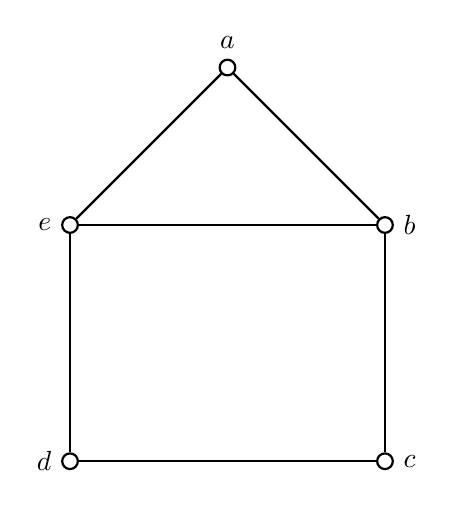
\begin{tikzpicture}
[nodedecorate/.style={shape=circle,inner sep=2pt,draw,thick},%
  linedecorate/.style={-,thick}]
% nodes or vertices
\node (a) at (0,5) [nodedecorate] {};
\node [above] at (a.north) {$a$};
\node (b) at (2,3) [nodedecorate] {};
\node [right] at (b.east) {$b$};
\node (e) at (-2,3) [nodedecorate] {};
\node [left] at (e.west) {$e$};
\node (c) at (2,0) [nodedecorate] {};
\node [right] at (c.east) {$c$};
\node (d) at (-2,0) [nodedecorate] {};
\node [left] at (d.west) {$d$};
% edges or lines
\path
(a) edge[linedecorate] node {} (b)
(b) edge[linedecorate] node {} (c)
(b) edge[linedecorate] node {} (e)
(c) edge[linedecorate] node {} (d)
(d) edge[linedecorate] node {} (e)
(e) edge[linedecorate] node {} (a);
\end{tikzpicture}
\caption{A house graph.}
\label{fig:introduction:house_graph}
\end{figure}

\begin{exercise}
\label{ex:introduction:house_graph}
Consider the graph in Figure~\ref{fig:introduction:house_graph}.
%
\begin{enumerate}
\item List the vertex and edge sets of the graph.

\item For each vertex, list all vertices that are adjacent to it.

\item Which vertex or vertices have the largest number of adjacent
  vertices? Similarly, which vertex or vertices have the smallest
  number of adjacent vertices?

\item If all edges of the graph are removed, is the resulting figure
  still a graph? Why or why not?

\item If all vertices of the graph are removed, is the resulting
  figure still a graph? Why or why not?
\end{enumerate}
\end{exercise}

\begin{proof}[Solution]
(1) Let $G = (V, E)$ denote the graph in
Figure~\ref{fig:introduction:house_graph}. Then the vertex set of $G$
is $V = \{ a, b, c, d, e \}$. The edge set of $G$ is given by
\begin{equation}
\label{eq:introduction:edges_of_house_graph}
E
=
\{ ab, ae, ba, bc, be, cb, cd, dc, de, ed, eb, ea \}.
\end{equation}
We can also use Sage to construct the graph $G$ and list its vertex
and edge sets:
%
\begin{center}
\fontsize{10pt}{10pt}
\selectfont
\tt
\begin{lstlisting}
sage: G = Graph({"a": ["b", "e"], "b": ["a", "c", "e"], "c": ["b", "d"], \
....: "d": ["c", "e"], "e": ["a", "b", "d"]})
sage: G
Graph on 5 vertices
sage: G.vertices()
['a', 'b', 'c', 'd', 'e']
sage: G.edges(labels=False)
[('a', 'b'), ('a', 'e'), ('b', 'e'), ('c', 'b'), ('c', 'd'), ('e', 'd')]
\end{lstlisting}
\end{center}
%
The graph $G$ is undirected, meaning that we do no impose direction on
any edges. Without any direction on the edges, the edge $ab$ is the
same as the edge $ba$. That is why \texttt{G.edges()} returns six
edges instead of the 12 edges listed
in~(\ref{eq:introduction:edges_of_house_graph}).

(2) Let $\text{adj}(v)$ be the set of all vertices that are adjacent
to $v$. Then we have
%
\begin{align*}
\text{adj}(a) &= \{ b, e \} \\
\text{adj}(b) &= \{ a, c, e \} \\
\text{adj}(c) &= \{ b, d \} \\
\text{adj}(d) &= \{ c, e \} \\
\text{adj}(e) &= \{ a, b, d \}
\end{align*}
%
The vertices adjacent to $v$ are also referred to as its
neighbours. We can use the function \texttt{G.neighbors()} to list all
the neighbours of each vertex.
%
\begin{center}
\fontsize{10pt}{10pt}
\selectfont
\tt
\begin{lstlisting}
sage: G.neighbors("a")
['b', 'e']
sage: G.neighbors("b")
['a', 'c', 'e']
sage: G.neighbors("c")
['b', 'd']
sage: G.neighbors("d")
['c', 'e']
sage: G.neighbors("e")
['a', 'b', 'd']
\end{lstlisting}
\end{center}

(3) Taking the cardinalities of the above five sets, we get
$|\text{adj}(a)| = |\text{adj}(c)| = |\text{adj}(d)| = 2$ and
$|\text{adj}(b)| = |\text{adj}(e)| = 3$. Thus $a$, $c$ and $d$ have
the smallest number of adjacent vertices, while $b$ and $e$ have the
largest number of adjacent vertices.

(4) If all the edges in $G$ are removed, the result is still a graph,
although one without any edges. By definition, the edge set of any
graph is a subset of $V \times V$. Removing all edges of $G$ leaves us
with the empty set $\emptyset$, which is a subset of every set.

(5) Say we remove all of the vertices from the graph in
Figure~\ref{fig:introduction:house_graph} and in the process all edges
are removed as well. The result is that both of the vertex and edge
sets are empty. This is a special graph known as an \emph{empty} or
\emph{null} graph.
\end{proof}

\begin{exercise}
Consider the illustration in
Figure~\ref{fig:introduction:self_loop}. Does
Figure~\ref{fig:introduction:self_loop} represent a graph? Why or why not?
\end{exercise}

\begin{proof}[Solution]
If $V = \{ a, b, c \}$ and $E = \{ aa, bc \}$, it is clear that $E
\subseteq V \times V$. Then $(V, E)$ is a graph. The edge $aa$ is
called a \emph{self-loop} of the graph. In general, any edge of the
form $vv$ is a self-loop.
\end{proof}

\begin{figure}[!htbp]
\centering
\begin{tikzpicture}
[nodedecorate/.style={shape=circle,inner sep=2pt,draw,thick},%
  arrowdecorate/.style={-,thick}]
% nodes or vertices
\node (c) at (-2,0) [nodedecorate] {};
\node [left] at (c.west) {$c$};
\node (b) at (2,0) [nodedecorate] {};
\node [right] at (b.east) {$b$};
\node (a) at (0,2) [nodedecorate] {};
\node [above] at (a.north) {$a$};
% edges or lines
\path
(a) edge[arrowdecorate,loop below,min distance=10mm,out=310,in=230] node {} (a)
(b) edge[arrowdecorate] node {} (c);
\end{tikzpicture}
\caption{A figure with a self-loop.}
\label{fig:introduction:self_loop}
\end{figure}

In Figure~\ref{fig:introduction:house_graph}, the edges $ae$ and $ea$
represent one and the same edge. If we do not consider the direction
of the edges in the graph of
Figure~\ref{fig:introduction:house_graph}, then the graph has six
edges. However, if the direction of each edge is taken into account,
then there are 12 edges as listed
in~(\ref{eq:introduction:edges_of_house_graph}). The following
definition captures the situation where the direction of the edges are
taken into account.

\begin{definition}
\textbf{Directed graphs.}
A \emph{directed edge} is an edge such that one vertex incident with it
is designated as the head vertex and the other incident vertex is
designated as the tail vertex. A directed edge is said to be directed
from its tail to its head. A \emph{directed graph} or \emph{digraph} is
a graph such that each of whose edges is directed.
\end{definition}
\index{graphs!directed}
\index{digraph}

It is important to distinguish a graph $G$ as being directed or
undirected. If $G$ is undirected and $uv \in E(G)$, then $uv$ and $vu$
represent the same edge. In case $G$ is a digraph, then $uv$ and $vu$
are different directed edges.

The edges of a digraph can be visually represented as directed arrows,
similarly to the digraph in
Figure~\ref{fig:introduction:directed_triangle_graph}. The graph in
Figure~\ref{fig:introduction:directed_triangle_graph} has the vertex
set $\{ a, b, c \}$ and the edge set $\{ ab, bc, ca \}$. There is an
arrow from vertex $a$ to vertex $b$, hence $ab$ is in the edge
set. However, there is no arrow from $b$ to $a$, so $ba$ is not in the
edge set of the graph in
Figure~\ref{fig:introduction:directed_triangle_graph}.

\begin{figure}[!htbp]
\centering
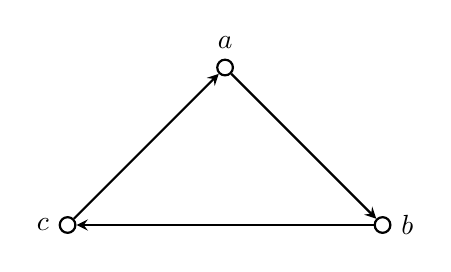
\begin{tikzpicture}
[nodedecorate/.style={shape=circle,inner sep=2pt,draw,thick},%
  arrowdecorate/.style={->,>=stealth,thick}]
% nodes or vertices
\node (c) at (-2,0) [nodedecorate] {};
\node [left] at (c.west) {$c$};
\node (b) at (2,0) [nodedecorate] {};
\node [right] at (b.east) {$b$};
\node (a) at (0,2) [nodedecorate] {};
\node [above] at (a.north) {$a$};
% edges or lines
\path
(a) edge[arrowdecorate] node {} (b)
(b) edge[arrowdecorate] node {} (c)
(c) edge[arrowdecorate] node {} (a);
\end{tikzpicture}
\caption{A triangle as a directed graph.}
\label{fig:introduction:directed_triangle_graph}
\end{figure}

For any vertex $v$ in a graph $G = (V, E)$, the cardinality of
$\text{adj}(v)$ is called the \emph{degree} of $v$ and written as
$\deg(v) = |\text{adj}(v)|$. The degree of $v$ counts the number of
vertices in $G$ that are adjacent to $v$. If $\deg(v) = 0$, we say
that $v$ is an \emph{isolated} vertex. For example, in the graph in
Figure~\ref{fig:introduction:house_graph}, we have $\deg(b) = 3$. For
the graph in Figure~\ref{fig:introduction:directed_triangle_graph}, we
have $\deg(b) = 2$. If $V \neq \emptyset$ and $E = \emptyset$, then
$G$ is a graph consisting entirely of isolated vertices. From
Exercise~\ref{ex:introduction:house_graph} we know that the vertices
$a, c, d$ in Figure~\ref{fig:introduction:house_graph} have the
smallest degree in the graph of that figure, while $b, e$ have the
largest degree. The minimum degree among all vertices in $G$ is
denoted $\delta(G)$, whereas the maximum degree is written as
$\Delta(G)$. Thus, if $G$ denotes the graph in
Figure~\ref{fig:introduction:house_graph} then we have $\delta(G) = 2$
and $\Delta(G) = 3$. In the following Sage session, we construct the
digraph in Figure~\ref{fig:introduction:directed_triangle_graph} and
computes its maximum and minimum number of degrees.
\index{degree of a vertex}

%
\begin{center}
\fontsize{10pt}{10pt}
\selectfont
\tt
\begin{lstlisting}
sage: G = DiGraph({"a": "b", "b": "c", "c": "a"})
sage: G
Digraph on 3 vertices
sage: G.degree("a")
2
sage: G.degree("b")
2
sage: G.degree("c")
2
\end{lstlisting}
\end{center}
%
So for the graph $G$ in
Figure~\ref{fig:introduction:directed_triangle_graph}, we have
$\delta(G) = \Delta(G) = 2$.

The graph $G$ in Figure~\ref{fig:introduction:directed_triangle_graph}
has the special property that its minimum degree is the same as its
maximum degree, i.e. $\delta(G) = \Delta(G)$. Graphs with this
property are referred to as \emph{regular}. An $r$-\emph{regular}
graph is a regular graph each of whose vertices has degree $r$. For
instance, $G$ is a $2$-regular graph. The following result, due to
Euler, counts the total number of degrees in any graph.
\index{graphs!regular}

\begin{theorem}
\label{thm:introduction:degree_sum}
\label{thm:introduction:hand_shaking}
\textbf{Euler.}
If $G = (V, E)$ is a graph, then $\sum_{v \in V} \deg(v) = 2 |E|$.
\end{theorem}
\index{hand-shaking lemma}

This lemma is sometimes called the ``hand-shaking lemma,'' due to its
interpretation as in the following story. Suppose you go into a
room. Suppose there are $n$ people in the room (including yourself)
and some people shake hands with others and some do not. Create the
graph with $n$ vertices, where each vertex is associated with a
different person. Draw an edge between two people if they shook
hands. The degree of a vertex is the number of times that person has
shaken hands (we assume that there are no multiple edges, i.e. that no
two people shake hands twice). The theorem above simply says that the
total number of hand shakes is even. This is ``obvious'' when you look
at it this way since each hand shake is counted twice ($A$ shaking
$B$'s hand is counted, $B$ shaking $A$'s hand, since the sum in the
theorem is over all vertices).

\begin{proof}
Each edge $e = v_1 v_2 \in E$ is incident with two vertices, so $e$ is
counted twice towards the total sum of degrees. The first time, we
count $e$ towards the degree of vertex $v_1$ and the second time we
count $e$ towards the degree of $v_2$.
\end{proof}

As $E \subseteq V \times V$, then $E$ can be the empty set, in which
case the total degree of $G = (V, E)$ is zero. Where $E \neq
\emptyset$, then the total degree of $G$ is greater than zero. By
Theorem~\ref{thm:introduction:degree_sum}, the total degree of $G$ is
non-negative and even. This result is an immediate consequence of
Theorem~\ref{thm:introduction:degree_sum} and is captured in the
following corollary.

\begin{corollary}
\label{cor:introduction:degree_sum_even}
If $G$ is a graph, then its total number of degrees is non-negative
and even.
\end{corollary}

If $G = (V, E)$ is an $r$-regular graph with $n$ vertices and $m$
edges, it is clear by definition of $r$-regular graphs that the total
degree of $G$ is $rn$. By Theorem~\ref{thm:introduction:degree_sum} we
have $2m = rn$ and therefore $m = rn / 2$. This result is captured in
the following corollary.

\begin{corollary}
If $G = (V, E)$ is an $r$-regular graph having $n$ vertices and $m$
edges, then $m = rn / 2$.
\end{corollary}


%%-----------------------------------------------------------------------%%
%%--- Subgraphs and other graph types -----------------------------------%%

\section{Subgraphs and other graph types}


%%-----------------------------------------------------------------------%%

\subsection{Walks, trails, and paths}

If $u$ and $v$ are two vertices in a graph $G$, a $u$-$v$ \emph{walk}
is an alternating sequence of vertices and edges starting with $u$ and
ending at $v$. Consecutive vertices and edges are incident. For the
graph in Figure~\ref{fig:introduction:types_of_walks}, an example of a
walk is an $a$-$e$ walk: $a, b, c, b, e$. In other words, we
start at vertex $a$ and travel to vertex $b$. From $b$, we go to $c$
and then back to $b$ again. Then we end our journey at $e$. Notice
that consecutive vertices in a walk are adjacent to each other. One
can think of vertices as destinations and edges as footpaths, say. We
are allowed to have repeated vertices and edges in a walk. The number
of edges in a walk is called its \emph{length}. For instance, the
walk $a, b, c, b, e$ has length $4$.
\index{walk, in a graph}

\begin{figure}[!htbp]
\centering
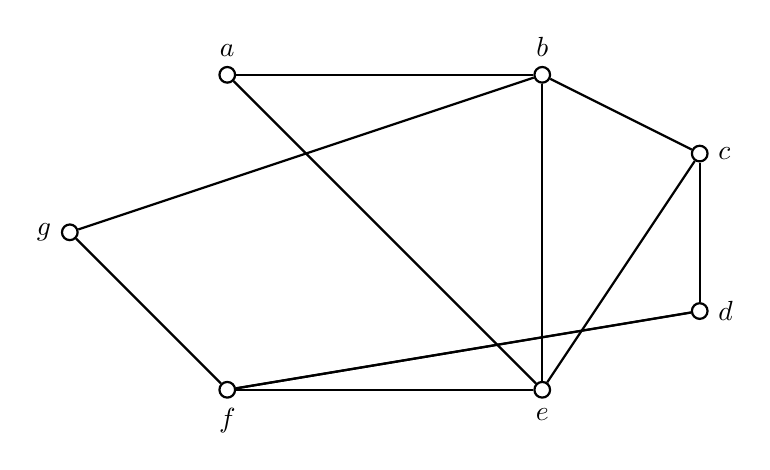
\begin{tikzpicture}
[nodedecorate/.style={shape=circle,inner sep=2pt,draw,thick},%
  linedecorate/.style={-,thick}]
% nodes or vertices
\node (b) at (4,4) [nodedecorate] {};
\node [above] at (b.north) {$b$};
\node (a) at (0,4) [nodedecorate] {};
\node [above] at (a.north) {$a$};
\node (c) at (6,3) [nodedecorate] {};
\node [right] at (c.east) {$c$};
\node (d) at (6,1) [nodedecorate] {};
\node [right] at (d.east) {$d$};
\node (e) at (4,0) [nodedecorate] {};
\node [below] at (e.south) {$e$};
\node (g) at (-2,2) [nodedecorate] {};
\node [left] at (g.west) {$g$};
\node (f) at (0,0) [nodedecorate] {};
\node [below] at (f.south) {$f$};
% edges or lines
\path
(a) edge[linedecorate] node {} (b)
(a) edge[linedecorate] node {} (e)
(b) edge[linedecorate] node {} (c)
(b) edge[linedecorate] node {} (e)
(b) edge[linedecorate] node {} (g)
(c) edge[linedecorate] node {} (d)
(c) edge[linedecorate] node {} (e)
(d) edge[linedecorate] node {} (f)
(d) edge[linedecorate] node {} (f)
(e) edge[linedecorate] node {} (f)
(f) edge[linedecorate] node {} (g);
\end{tikzpicture}
\caption{Walking along a graph.}
\label{fig:introduction:types_of_walks}
\end{figure}

A \emph{trail} is a walk with no repeating edges. For example, the
$a$-$b$ walk $a, b, c, d, f, g, b$ in
Figure~\ref{fig:introduction:types_of_walks} is a trail. It does not
contain any repeated edges, but it contains one repeated vertex,
i.e. $b$. Nothing in the definition of a trail restricts a trail from
having repeated vertices. 
\index{trail}
%\index{circuit}
\index{path}
\index{cycle}

A walk with no repeating vertices is called a \emph{path}. Without any
repeating vertices, a path cannot have repeating edges, hence a path
is also a trail. A path whose start and end vertices are the same is
called a \emph{cycle}. For example, the walk $a, b, c, e, a$
in Figure~\ref{fig:introduction:types_of_walks} is a path and a cycle.
A walk which has no repeated edges and 
the start and end vertices are the same, but otherwise has no 
repeated vertices, is 
%a \emph{circuit}, otherwise known as 
a \emph{closed path} (with apologies for
slightly abusing terminology)\footnote{A closed path in a graph is
 sometimes also called a circuit. Since that terminology 
unfortunately conflicts with the closely related notion of a circuit
of a matroid, we do not use it here.}. Thus the walk $a, b, e, a$ 
in Figure~\ref{fig:introduction:types_of_walks} is a
closed path. It is easy to see that if you remove any edge
from a cycle then the resulting walk contains no closed paths.

\begin{exercise}
Consider the graph in Figure~\ref{fig:introduction:types_of_walks}.
%
\begin{enumerate}
\item Find two distinct walks that are not trails and determine their
  lengths.

\item Find two distinct trails that are not paths and determine their
  lengths.

\item Find two distinct paths and determine their lengths.

\item Find a closed path that is not a cycle.

\item
Find a closed path $C$ which has an edge $e$ such that
$C-e$ contains a cycle.
\end{enumerate}
\end{exercise}

\begin{proof}[Solution]
(1) Here are two distinct walks that are not trails:
$w_1: g, b, e, a, b, e$ and $w_2: f, d, c, e, f, d$. The length of
walk $w_1$ is 5 and the length of walk $w_2$ is also 5.

(2) Here are two distinct trails that are not paths:
$t_1: a, b, c, d, f$ and $t_2: b, e, f, d, c$. The length of trail
$t_1$ is 4 and the length of trail $t_2$ is also 4.

(3) Here are two distinct paths: $p_1: a, b, c, d, f, e$ and
$p_2: g, b, a, e, f, d$. The length of path $p_1$ is 5 and the length
of path $p_2$ is also 5.

(4) Here is a closed path that is not a cycle: $d, c, e, b, a, e, f, d$.
\end{proof}

A graph is said to be \emph{connected} if for every pair of distinct
vertices $u, v$ there is a $u$-$v$ path joining them. A graph that is
not connected is referred to as \emph{disconnected}. The empty graph
is disconnected and so is any non-empty graph with an isolated
vertex. However, the graph in
Figure~\ref{fig:introduction:directed_triangle_graph} is
connected. A \emph{geodesic path} or \emph{shortest path} between two
distinct vertices $u,v$ of a graph is a $u$-$v$ path of minimum
length. A non-empty graph may have several shortest paths between some
distinct pair of vertices. For the graph in
Figure~\ref{fig:introduction:types_of_walks}, both $a,b,c$ and $a,e,c$
are geodesic paths between $a$ and $c$.
\index{path!geodesic}
\index{graph!connected}

\begin{exercise}
Determine whether or not the graph in
Figure~\ref{fig:introduction:types_of_walks} is connected. Find a
shortest path from $g$ to $d$.
\end{exercise}

\begin{proof}[Solution]
In the following Sage session, we first construct the graph in
Figure~\ref{fig:introduction:types_of_walks} and use the method
\verb!is_connected()! to determine whether or not the graph is
connected. Finally, we use the method \verb!shortest_path()! to find
a geodesic path between $g$ and $d$.
%
\begin{center}
\fontsize{10pt}{10pt}
\selectfont
\tt
\begin{lstlisting}
sage: g = Graph({"a": ["b", "e"], "b": ["a", "g", "e", "c"], \
....: "c": ["b", "e", "d"], "d": ["c", "f"], "e": ["f", "a", "b", "c"], \
....: "f": ["g", "d", "e"], "g": ["b", "f"]})
sage: g.is_connected()
True
sage: g.shortest_path("g", "d")
['g', 'f', 'd']
\end{lstlisting}
\end{center}
%
This shows that $g, f, d$ is a shortest path from $g$ to $d$. In fact,
any other $g$-$d$ path has length greater than $2$, so we can say that
$g, f, d$ is the shortest path between $g$ and $d$.
\end{proof}

We will explain Dijkstra's algorithm in
Chapter~\ref{chap:graph_algorithms}, which gives one of the best
algorithms for finding shortest paths between two vertices in a
connected graph. What is very remarkable is that, at the present state
of knowledge, finding the shortest path from a vertex $v$ to a
\emph{particular} (but arbitrarily given) vertex $w$ appears to be as
hard as finding the shortest path from a vertex $v$ to \emph{all}
other vertices in the graph!


%%-----------------------------------------------------------------------%%

\subsection{Subgraphs, complete and bipartite graphs}

\begin{definition}
Let $G$ be a graph with vertex set $V(G)$ and edge set
$E(G)$. Consider a graph $H$ such that $V(H) \subseteq V(G)$ and $E(H)
\subseteq E(G)$. Furthermore, if $uv \in E(H)$ then $u,v \in
V(H)$. Then $H$ is called a \emph{subgraph} of $G$ and $G$ is referred
to as a \emph{supergraph} of $H$.
\end{definition}
\index{subgraph}
\index{supergraph}

Starting from $G$, one can obtain its subgraph $H$ by deleting edges
and/or vertices from $G$. Note that when a vertex $v$ is removed from
$G$, then all edges incident with $v$ are also removed. If $V(H) =
V(G)$, then $H$ is called a \emph{spanning} subgraph of $G$. In
Figure~\ref{fig:introduction:star_subgraph}, let $G$ be the left-hand
side graph and let $H$ be the right-hand side graph. Then it is clear
that $H$ is a spanning subgraph of $G$. To obtain a spanning subgraph
from a given graph, we delete edges from the given graph.
\index{spanning subgraph}

\begin{figure}[!htbp]
\centering
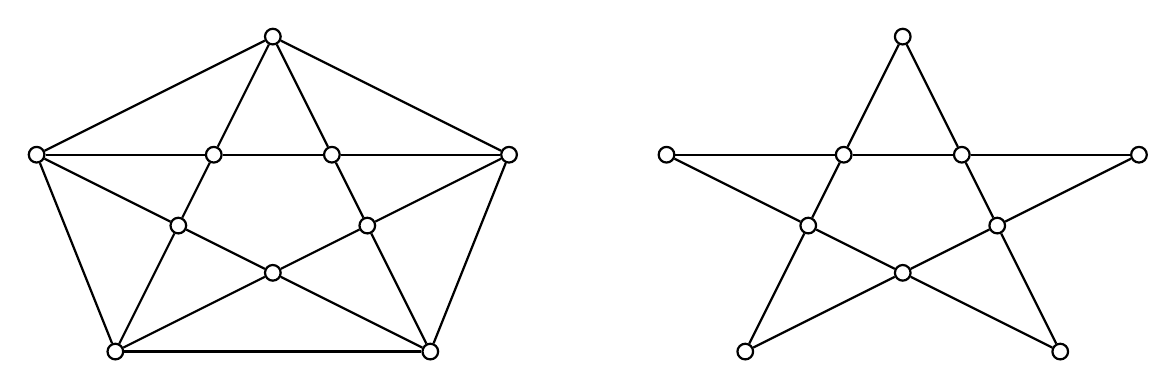
\begin{tikzpicture}
[nodedecorate/.style={shape=circle,inner sep=2pt,draw,thick},%
  linedecorate/.style={-,thick}]
%%% pentagon with star and inner pentagon
% nodes or vertices
\node (a) at (-2,0) [nodedecorate] {};
\node (b) at (2,0) [nodedecorate] {};
\node (c) at (-3,2.5) [nodedecorate] {};
\node (d) at (3,2.5) [nodedecorate] {};
\node (e) at (0,4) [nodedecorate] {};
\node (f) at (-0.75,2.5) [nodedecorate] {};
\node (g) at (-1.2,1.6) [nodedecorate] {};
\node (h) at (0,1) [nodedecorate] {};
\node (i) at (1.2,1.6) [nodedecorate] {};
\node (j) at (0.75,2.5) [nodedecorate] {};
% edges or lines
\path
(a) edge[linedecorate] node {} (b)
(a) edge[linedecorate] node {} (c)
(a) edge[linedecorate] node {} (g)
(a) edge[linedecorate] node {} (h)
(b) edge[linedecorate] node {} (d)
(b) edge[linedecorate] node {} (h)
(b) edge[linedecorate] node {} (i)
(c) edge[linedecorate] node {} (e)
(c) edge[linedecorate] node {} (f)
(c) edge[linedecorate] node {} (g)
(d) edge[linedecorate] node {} (e)
(d) edge[linedecorate] node {} (i)
(d) edge[linedecorate] node {} (j)
(e) edge[linedecorate] node {} (f)
(e) edge[linedecorate] node {} (j)
(f) edge[linedecorate] node {} (g)
(f) edge[linedecorate] node {} (j)
(g) edge[linedecorate] node {} (h)
(h) edge[linedecorate] node {} (i)
(i) edge[linedecorate] node {} (j);
%
%%% star and inner pentagon
% nodes or vertices
\node (a2) at (6,0) [nodedecorate] {};
\node (b2) at (10,0) [nodedecorate] {};
\node (c2) at (5,2.5) [nodedecorate] {};
\node (d2) at (11,2.5) [nodedecorate] {};
\node (e2) at (8,4) [nodedecorate] {};
\node (f2) at (7.25,2.5) [nodedecorate] {};
\node (g2) at (6.8,1.6) [nodedecorate] {};
\node (h2) at (8,1) [nodedecorate] {};
\node (i2) at (9.2,1.6) [nodedecorate] {};
\node (j2) at (8.75,2.5) [nodedecorate] {};
% edges or lines
\path
(a2) edge[linedecorate] node {} (g2)
(a2) edge[linedecorate] node {} (h2)
(b2) edge[linedecorate] node {} (h2)
(b2) edge[linedecorate] node {} (i2)
(c2) edge[linedecorate] node {} (f2)
(c2) edge[linedecorate] node {} (g2)
(d2) edge[linedecorate] node {} (i2)
(d2) edge[linedecorate] node {} (j2)
(e2) edge[linedecorate] node {} (f2)
(e2) edge[linedecorate] node {} (j2)
(f2) edge[linedecorate] node {} (g2)
(f2) edge[linedecorate] node {} (j2)
(g2) edge[linedecorate] node {} (h2)
(h2) edge[linedecorate] node {} (i2)
(i2) edge[linedecorate] node {} (j2);
\end{tikzpicture}
\caption{A graph and one of its subgraphs.}
\label{fig:introduction:star_subgraph}
\end{figure}

\index{graph!complete}
We now consider several standard classes of graphs. The \emph{complete}
graph $K_n$ on $n$ vertices is a graph such that any two distinct
vertices are adjacent. As $|V(K_n)| = n$, then $|E(K_n)|$ is
equivalent to the total number of 2-combinations from a set of $n$
objects:
\[
|E(K_n)|
=
\binom{n}{2}
=
\frac{n(n-1)}{2}
\]
Thus for any graph $G$ with $n$ vertices, its total number of edges
$|E(G)|$ is bounded above by
\[
|E(G)|
\leq
\frac{n(n - 1)}{2}
\]
Figure~\ref{fig:introduction:five_complete_graphs} shows complete
graphs each of whose total number of vertices is bounded by
$1 \leq n \leq 5$. The complete graph $K_1$ has one vertex with
no edges. It is also called the \emph{trivial} graph.
\index{graph!trivial}

\begin{figure}[!htbp]
\centering
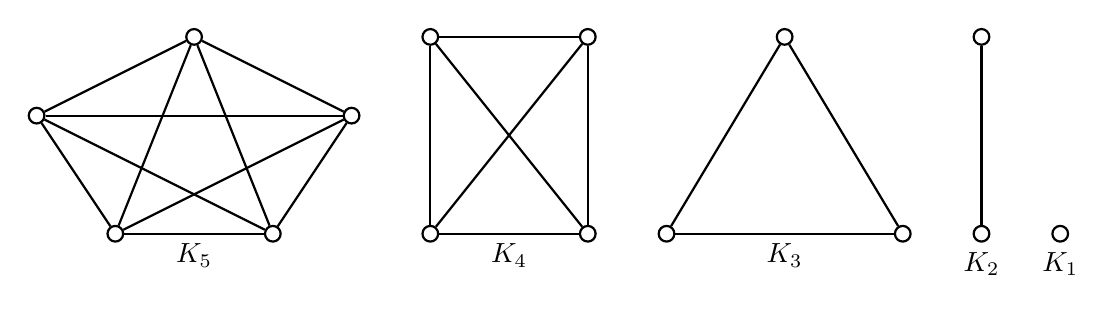
\begin{tikzpicture}
[nodedecorate/.style={shape=circle,inner sep=2pt,draw,thick},%
  linedecorate/.style={-,thick}]
%%% complete graph K_5
% nodes or vertices
\node (a) at (-1,0) [nodedecorate] {};
\node (b) at (1,0) [nodedecorate] {};
\node (c) at (-2,1.5) [nodedecorate] {};
\node (d) at (2,1.5) [nodedecorate] {};
\node (e) at (0,2.5) [nodedecorate] {};
% edges or lines
\path
(a) edge[linedecorate] node[below] {$K_5$} (b)
(a) edge[linedecorate] node {} (c)
(a) edge[linedecorate] node {} (d)
(a) edge[linedecorate] node {} (e)
(b) edge[linedecorate] node {} (c)
(b) edge[linedecorate] node {} (d)
(b) edge[linedecorate] node {} (e)
(c) edge[linedecorate] node {} (d)
(c) edge[linedecorate] node {} (e)
(d) edge[linedecorate] node {} (e);
%
%%% complete graph K_4
% nodes or vertices
\node (a) at (3,0) [nodedecorate] {};
\node (b) at (5,0) [nodedecorate] {};
\node (c) at (3,2.5) [nodedecorate] {};
\node (d) at (5,2.5) [nodedecorate] {};
% edges or lines
\path
(a) edge[linedecorate] node[below] {$K_4$} (b)
(a) edge[linedecorate] node {} (c)
(a) edge[linedecorate] node {} (d)
(b) edge[linedecorate] node {} (c)
(b) edge[linedecorate] node {} (d)
(c) edge[linedecorate] node {} (d);
%
%%% complete graph K_3
% nodes or vertices
\node (a) at (6,0) [nodedecorate] {};
\node (b) at (9,0) [nodedecorate] {};
\node (c) at (7.5,2.5) [nodedecorate] {};
% edges or lines
\path
(a) edge[linedecorate] node[below] {$K_3$} (b)
(a) edge[linedecorate] node {} (c)
(b) edge[linedecorate] node {} (c);
%
%%% complete graph K_2
% nodes or vertices
\node (a) at (10,0) [nodedecorate] {};
\node [below] at (a.south) {$K_2$};
\node (b) at (10,2.5) [nodedecorate] {};
% edges or lines
\path
(a) edge[linedecorate] node {} (b);
%
%%% complete graph K_1
% nodes or vertices
\node (a) at (11,0) [nodedecorate] {};
\node [below] at (a.south) {$K_1$};
\end{tikzpicture}
\caption{Complete graphs $K_n$ for $1 \leq n \leq 5$.}
\label{fig:introduction:five_complete_graphs}
\end{figure}

\index{graph!cycle}
The \emph{cycle} graph on $n \geq 3$ vertices, denoted $C_n$, is the
connected $2$-regular graph on $n$ vertices. Each vertex in $C_n$ has
degree exactly $2$ and $C_n$ is
connected. Figure~\ref{fig:introduction:four_cycle_graphs} shows
cycles graphs $C_n$ where $3 \leq n \leq 6$. The \emph{path} on
$n \geq 1$ vertices is denoted $P_n$. For $n = 1, 2$ we have
$P_1 = K_1$ and $P_2 = K_2$. Where $n \geq 3$, then $P_n$ is a
spanning subgraph of $C_n$ obtained by deleting one edge.

\begin{figure}[!htbp]
\centering
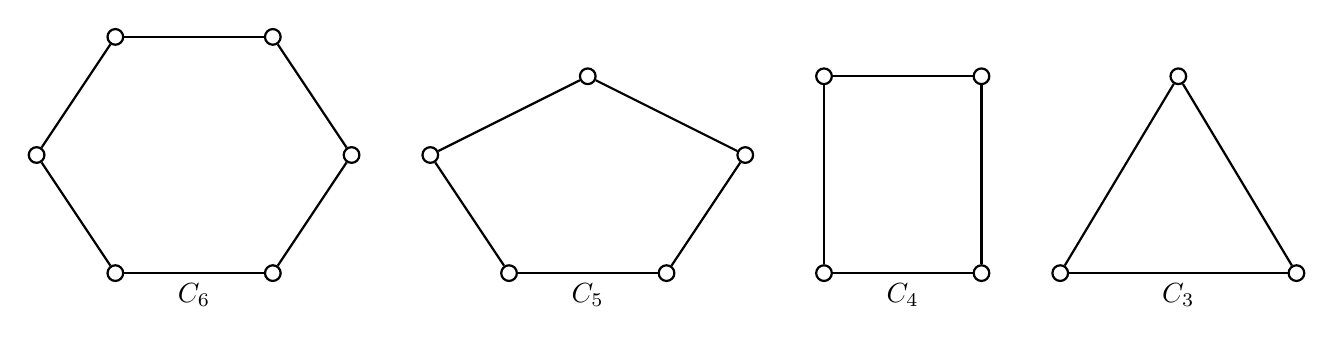
\begin{tikzpicture}
[nodedecorate/.style={shape=circle,inner sep=2pt,draw,thick},%
  linedecorate/.style={-,thick}]
%%% cycle graph C_6
% nodes or vertices
\node (a) at (-6,0) [nodedecorate] {};
\node (b) at (-4,0) [nodedecorate] {};
\node (c) at (-7,1.5) [nodedecorate] {};
\node (d) at (-3,1.5) [nodedecorate] {};
\node (e) at (-6,3) [nodedecorate] {};
\node (f) at (-4,3) [nodedecorate] {};
% edges or lines
\path
(a) edge[linedecorate] node[below] {$C_6$} (b)
(a) edge[linedecorate] node {} (c)
(b) edge[linedecorate] node {} (d)
(c) edge[linedecorate] node {} (e)
(d) edge[linedecorate] node {} (f)
(e) edge[linedecorate] node {} (f);
%
%%% cycle graph C_5
% nodes or vertices
\node (a) at (-1,0) [nodedecorate] {};
\node (b) at (1,0) [nodedecorate] {};
\node (c) at (-2,1.5) [nodedecorate] {};
\node (d) at (2,1.5) [nodedecorate] {};
\node (e) at (0,2.5) [nodedecorate] {};
% edges or lines
\path
(a) edge[linedecorate] node[below] {$C_5$} (b)
(a) edge[linedecorate] node {} (c)
(b) edge[linedecorate] node {} (d)
(c) edge[linedecorate] node {} (e)
(d) edge[linedecorate] node {} (e);
%
%%% cycle graph C_4
% nodes or vertices
\node (a) at (3,0) [nodedecorate] {};
\node (b) at (5,0) [nodedecorate] {};
\node (c) at (3,2.5) [nodedecorate] {};
\node (d) at (5,2.5) [nodedecorate] {};
% edges or lines
\path
(a) edge[linedecorate] node[below] {$C_4$} (b)
(a) edge[linedecorate] node {} (c)
(b) edge[linedecorate] node {} (d)
(c) edge[linedecorate] node {} (d);
%
%%% cycle graph C_3
% nodes or vertices
\node (a) at (6,0) [nodedecorate] {};
\node (b) at (9,0) [nodedecorate] {};
\node (c) at (7.5,2.5) [nodedecorate] {};
% edges or lines
\path
(a) edge[linedecorate] node[below] {$C_3$} (b)
(a) edge[linedecorate] node {} (c)
(b) edge[linedecorate] node {} (c);
\end{tikzpicture}
\caption{Cycle graphs $C_n$ for $3 \leq n \leq 6$.}
\label{fig:introduction:four_cycle_graphs}
\end{figure}

A \emph{bipartite} graph $G$ is a graph with at least two
vertices such that $V(G)$ can be split into two disjoint subsets $V_1$
and $V_2$, both non-empty. Every edge $uv \in E(G)$ is such that
$u \in V_1$ and $v \in V_2$, or $v \in V_1$ and $u \in V_2$. The
\emph{complete bipartite} graph $K_{m,n}$ is the bipartite graph whose
vertex set is partitioned into two non-empty disjoint sets $V_1$ and
$V_2$ with $|V_1| = m$ and $|V_2| = n$. Any vertex in $V_1$ is
adjacent to each vertex in $V_2$, and any two distinct vertices in
$V_i$ are not adjacent to each other. If $m = n$, then $K_{n,n}$ is
$n$-regular. Where $m = 1$ then $K_{1,n}$ is called the \emph{star}
graph. Figure~\ref{fig:introduction:bipartite_complete_bipartite_graphs}
shows a bipartite graph together with the complete bipartite graphs
$K_{4,3}$ and $K_{3,3}$, and the star graph $K_{1,4}$.

\begin{figure}[!htbp]
\centering
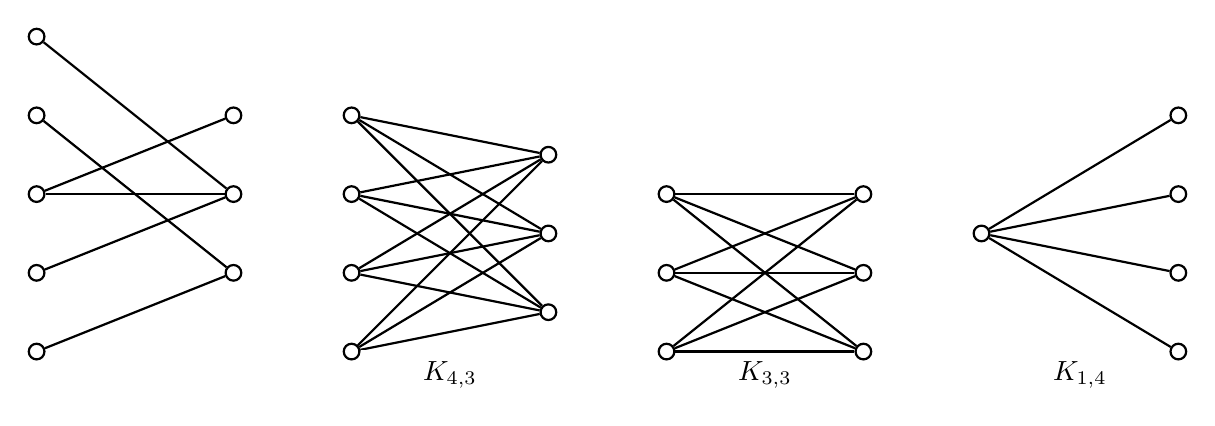
\begin{tikzpicture}
[nodedecorate/.style={shape=circle,inner sep=2pt,draw,thick},%
  linedecorate/.style={-,thick}]
%%% bipartite graph
% nodes or vertices
\node (a) at (0,0) [nodedecorate] {};
\node (b) at (0,1) [nodedecorate] {};
\node (c) at (0,2) [nodedecorate] {};
\node (d) at (0,3) [nodedecorate] {};
\node (e) at (0,4) [nodedecorate] {};
\node (f) at (2.5,3) [nodedecorate] {};
\node (g) at (2.5,2) [nodedecorate] {};
\node (h) at (2.5,1) [nodedecorate] {};
% edges or lines
\path
(a) edge[linedecorate] node {} (h)
(b) edge[linedecorate] node {} (g)
(c) edge[linedecorate] node {} (g)
(c) edge[linedecorate] node {} (f)
(d) edge[linedecorate] node {} (h)
(e) edge[linedecorate] node {} (g);
%
%%% complete bipartite graph K_{4,3}
% nodes or vertices
\node (a) at (4,0) [nodedecorate] {};
\node (b) at (4,1) [nodedecorate] {};
\node (c) at (4,2) [nodedecorate] {};
\node (d) at (4,3) [nodedecorate] {};
\node (e) at (6.5,2.5) [nodedecorate] {};
\node (f) at (6.5,1.5) [nodedecorate] {};
\node (g) at (6.5,0.5) [nodedecorate] {};
\node (h) at (6.5,0) [nodedecorate,color=white] {};
% edges or lines
\path
(a) edge[linedecorate] node {} (e)
(a) edge[linedecorate] node {} (f)
(a) edge[linedecorate] node {} (g)
(a) edge[linedecorate,color=white] node[below,color=black] {$K_{4,3}$} (h)
(b) edge[linedecorate] node {} (e)
(b) edge[linedecorate] node {} (f)
(b) edge[linedecorate] node {} (g)
(c) edge[linedecorate] node {} (e)
(c) edge[linedecorate] node {} (f)
(c) edge[linedecorate] node {} (g)
(d) edge[linedecorate] node {} (e)
(d) edge[linedecorate] node {} (f)
(d) edge[linedecorate] node {} (g);
%
%%% complete bipartite graph K_{3,3}
% nodes or vertices
\node (a) at (8,0) [nodedecorate] {};
\node (b) at (8,1) [nodedecorate] {};
\node (c) at (8,2) [nodedecorate] {};
\node (d) at (10.5,2) [nodedecorate] {};
\node (e) at (10.5,1) [nodedecorate] {};
\node (f) at (10.5,0) [nodedecorate] {};
% edges or lines
\path
(a) edge[linedecorate] node {} (d)
(a) edge[linedecorate] node {} (e)
(a) edge[linedecorate] node[below] {$K_{3,3}$} (f)
(b) edge[linedecorate] node {} (d)
(b) edge[linedecorate] node {} (e)
(b) edge[linedecorate] node {} (f)
(c) edge[linedecorate] node {} (d)
(c) edge[linedecorate] node {} (e)
(c) edge[linedecorate] node {} (f);
%
%%% star graph K_{1,4}
% nodes or vertices
\node (a) at (12,1.5) [nodedecorate] {};
\node (b) at (14.5,3) [nodedecorate] {};
\node (c) at (14.5,2) [nodedecorate] {};
\node (d) at (14.5,1) [nodedecorate] {};
\node (e) at (14.5,0) [nodedecorate] {};
\node (f) at (12,0) [nodedecorate,color=white] {};
% edges or lines
\path
(a) edge[linedecorate] node {} (b)
(a) edge[linedecorate] node {} (c)
(a) edge[linedecorate] node {} (d)
(a) edge[linedecorate] node {} (e)
(f) edge[linedecorate,color=white] node[below,color=black] {$K_{1,4}$} (e);
\end{tikzpicture}
\caption{Bipartite, complete bipartite and star graphs.}
\label{fig:introduction:bipartite_complete_bipartite_graphs}
\end{figure}

As an example of $K_{3,3}$, suppose that there are $3$ boys and $3$
girls dancing in a room. The boys and girls naturally partition the
set of all people in the room. Construct a graph having $6$ vertices,
each vertex corresponding to a person in the room, and draw an edge
form one vertex to another if the two people dance together. If each
girl dances three times, once with with each of the three boys, then
the resulting graph is $K_{3,3}$.

%%--- Representing graphs as matrices -----------------------------------%%

\section{Representing graphs as matrices}

Representing a graph as a matrix is very inefficient in some cases
and not so in other cases. For example, if you walk into a large room
full of people and you consider the ``hand-shaking graph'' that we
discussed in connection with
Theorem~\ref{thm:introduction:hand_shaking}. If not many people shake
hands in the room, then it is a waste of time to have to record all
the hand-shakes and also all the ``non-hand-shakes.'' This is
basically what the adjacency matrix does. In this kind of ``sparse
graph'' situation, it would
be much easier to simply record the hand-shakes as a Python dictionary.

If $G$ is an undirected graph with vertices $V=\{v_1,\dots, v_n\}$
and edges $E$ then the 
{\it adjacency matrix} of $G$ is the $n\times n$ matrix $A=(a_{ij})$ 
defined by

\[
a_{ij}=
\left\{
\begin{array}{ll}
1, & {\rm if}\ (v_i,v_j)\in E,\\
0, &{\rm otherwise}.
\end{array}
\right.
\]
If $G$ is an undirected graph then $A$ 
is a symmetric matrix.

If $G$ is a directed graph with vertices $V=\{v_1,\dots, v_n\}$
and edges $E$ then the $(0,-1,1)$-{\it adjacency matrix} 
of $G$ is the $n\times n$ matrix $A=(a_{ij})$ 
defined by
\index{adjacency matrix} 

\[
a_{ij}=
\left\{
\begin{array}{rl}
1, & {\rm if}\ (v_i,v_j)\in E,\\
-1, & {\rm if}\ (v_j,v_i)\in E,\\
0, &{\rm otherwise}.
\end{array}
\right.
\]

%\begin{itemize}
%\item what's a matrix?
%
%\item adjacency matrices for digraphs
%
%\item adjacency matrices for undirected graphs
%\end{itemize}

%\begin{example}
For example, Sage allows you to easily compute an adjacency matrix.

%
\begin{center}
\fontsize{10pt}{10pt}
\selectfont
\tt
\begin{lstlisting}
sage: C6 = Graph({1: [2, 4], 2: [1, 3], 3: [2, 6], 4: [1, 5], \
....: 5: [4, 6], 6: [3, 5]})
sage: G1 = Graph({"a": ["b", "c"], "b": ["a", "d"], "c": ["a", "e"], \
....: "d": ["b", "f"], "e": ["c", "f"], "f": ["d", "e"]})
sage: G1.adjacency_matrix()
[0 1 0 1 0 0]
[1 0 1 0 0 0]
[0 1 0 0 0 1]
[1 0 0 0 1 0]
[0 0 0 1 0 1]
[0 0 1 0 1 0]
sage: G2.adjacency_matrix()
[0 1 1 0 0 0]
[1 0 0 1 0 0]
[1 0 0 0 1 0]
[0 1 0 0 0 1]
[0 0 1 0 0 1]
[0 0 0 1 1 0]
sage: G1.adjacency_matrix()^2
[2 0 1 0 1 0]
[0 2 0 1 0 1]
[1 0 2 0 1 0]
[0 1 0 2 0 1]
[1 0 1 0 2 0]
[0 1 0 1 0 2]
\end{lstlisting}
\end{center}
%
%\end{example}


\begin{theorem}
Let $G$ be a graph of order $n$ and $\mathbf{A}$ the adjacency matrix
of $G$. For each positive integer $k$, the $i$-$j$ entry of
$\mathbf{A}^k$ counts the number of $v_i$-$v_j$ walks of length $k$.
\end{theorem}

There is an analog of the adjacency matrix for edges.
If $G$ is an undirected graph with edges $E=\{e_1,\dots, e_m\}$
and vertices $V=\{v_1,\dots,v_m\}$ then the 
{\it incidence matrix} of $G$ is the $n\times m$ matrix $B=(b_{ij})$ 
defined by

\[
b_{ij}=
\left\{
\begin{array}{ll}
1, & {\rm if}\ v_i\ {\rm incident\ to}\ e_j,\\
0, &{\rm otherwise}.
\end{array}
\right.
\]
If $G$ is a directed graph with edges $E=\{e_1,\dots, e_m\}$
and vertices $V=\{v_1,\dots,v_m\}$ then the 
{\it incidence matrix} of $G$ is the $n\times m$ matrix $B=(b_{ij})$ 
defined by
\index{incidence matrix}

\[
b_{ij}=
\left\{
\begin{array}{rl}
-1, & {\rm if}\ v_i\ {\rm incident\ to}\ e_j,\ e_j \ {\rm leaves}\
v_i\\
1, & {\rm if}\ v_i\ {\rm incident\ to}\ e_j,\ e_j \ {\rm enters}\ v_i\\
0, &{\rm otherwise}.
\end{array}
\right.
\]

Sage allows you to compute the incidence matrix of a 
graph.

%\begin{example}
%
\begin{center}
\fontsize{9pt}{9pt}
\selectfont
\tt
\begin{lstlisting}
sage: G = Graph({1: [2, 4], 2: [1, 3], 3: [2, 6], 4: [1, 5], 5: [4, 6], 6: [3, 5]})
sage: G.incidence_matrix()
[-1 -1  0  0  0  0]
[ 0  1 -1  0  0  0]
[ 0  0  1 -1  0  0]
[ 1  0  0  0 -1  0]
[ 0  0  0  0  1 -1]
[ 0  0  0  1  0  1]
\end{lstlisting}
\end{center}
%
%\end{example}


%%-----------------------------------------------------------------------%%
%%--- Isomorphic graphs -------------------------------------------------%%

\section{Isomorphic graphs}

Determining whether or not two graphs are, in some sense, the ``same''
is a hard but important problem.

\begin{definition}
\textbf{Isomorphic graphs.}
Two graphs $G$ and $H$ are \emph{isomorphic} if there is a bijection
$f: V(G) \longrightarrow V(H)$ such that whenever $uv \in E(G)$ then
$f(u) f(v) \in E(H)$. The function $f$ is an \emph{isomorphism}
between $G$ and $H$. Otherwise, $G$ and $H$ are non-isomorphic. If
$G$ and $H$ are isomorphic, we write $G \cong H$.
\end{definition}
\index{graphs!isomorphic}

A graph $G$ is isomorphic to a graph $H$ if these two graphs can be
labelled in such a way that if $u$ and $v$ are adjacent in $G$, then
their counterparts in $V(H)$ are also adjacent in $H$. To determine
whether or not two graphs are isomorphic is to determine if they are
structurally equivalent. Graphs $G$ and $H$ may be drawn differently
so that they seem different. However, if $G \cong H$ then the
isomorphism $f: V(G) \longrightarrow V(H)$ shows that both of these
graphs are fundamentally the same. In particular, the order and size
of $G$ are equal to those of $H$, the isomorphism $f$ preserves
adjacencies, and $\deg(v) = \deg(f(v))$ for all $v \in G$. Since $f$
preserves adjacencies, then adjacencies along a given geodesic path
are preserved as well. That is, if $v_1, v_2, v_3, \dots, v_k$ is a
shortest path between $v_1, v_k \in V(G)$, then
$f(v_1), f(v_2), f(v_3), \dots, f(v_k)$ is a geodesic path between
$f(v_1), f(v_k) \in V(H)$.

%% Hopefully later we can discuss ``canonical labeling''
%% and how that gives rise to isomorphism/automorphism
%% testing methods???

\begin{figure}[!htbp]
\centering
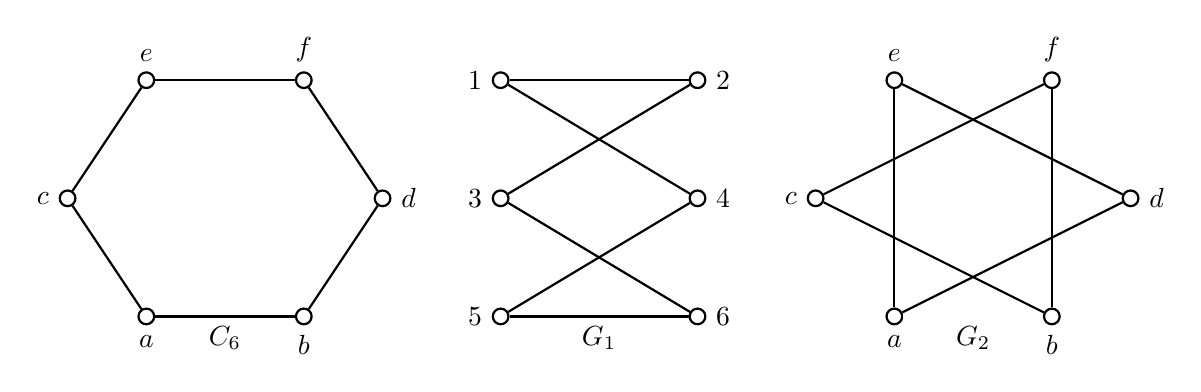
\begin{tikzpicture}
[nodedecorate/.style={shape=circle,inner sep=2pt,draw,thick},%
  linedecorate/.style={-,thick}]
%%% cycle graph C_6
% nodes or vertices
\node (a) at (0,0) [nodedecorate] {};
\node [below] at (a.south) {$a$};
\node (b) at (2,0) [nodedecorate] {};
\node [below] at (b.south) {$b$};
\node (c) at (-1,1.5) [nodedecorate] {};
\node [left] at (c.west) {$c$};
\node (d) at (3,1.5) [nodedecorate] {};
\node [right] at (d.east) {$d$};
\node (e) at (0,3) [nodedecorate] {};
\node [above] at (e.north) {$e$};
\node (f) at (2,3) [nodedecorate] {};
\node [above] at (f.north) {$f$};
% edges or lines
\path
(a) edge[linedecorate] node[below] {$C_6$} (b)
(a) edge[linedecorate] node {} (c)
(b) edge[linedecorate] node {} (d)
(c) edge[linedecorate] node {} (e)
(d) edge[linedecorate] node {} (f)
(e) edge[linedecorate] node {} (f);
%
%%% graph G_1 that is isomorphic to C_6
% nodes or vertices
\node (1) at (4.5,3) [nodedecorate] {};
\node [left] at (1.west) {$1$};
\node (2) at (7,3) [nodedecorate] {};
\node [right] at (2.east) {$2$};
\node (3) at (4.5,1.5) [nodedecorate] {};
\node [left] at (3.west) {$3$};
\node (4) at (7,1.5) [nodedecorate] {};
\node [right] at (4.east) {$4$};
\node (5) at (4.5,0) [nodedecorate] {};
\node [left] at (5.west) {$5$};
\node (6) at (7,0) [nodedecorate] {};
\node [right] at (6.east) {$6$};
% edges or lines
\path
(1) edge[linedecorate] node {} (2)
(1) edge[linedecorate] node {} (4)
(3) edge[linedecorate] node {} (2)
(3) edge[linedecorate] node {} (6)
(5) edge[linedecorate] node {} (4)
(5) edge[linedecorate] node[below] {$G_1$} (6);
%
%%% graph G_2 that is non-isomorphic to C_6
% nodes or vertices
\node (a) at (9.5,0) [nodedecorate] {};
\node [below] at (a.south) {$a$};
\node (b) at (11.5,0) [nodedecorate] {};
\node [below] at (b.south) {$b$};
\node (c) at (8.5,1.5) [nodedecorate] {};
\node [left] at (c.west) {$c$};
\node (d) at (12.5,1.5) [nodedecorate] {};
\node [right] at (d.east) {$d$};
\node (e) at (9.5,3) [nodedecorate] {};
\node [above] at (e.north) {$e$};
\node (f) at (11.5,3) [nodedecorate] {};
\node [above] at (f.north) {$f$};
% edges or lines
\path
(a) edge[linedecorate] node {} (d)
(a) edge[linedecorate] node {} (e)
(b) edge[linedecorate] node {} (c)
(b) edge[linedecorate] node {} (f)
(c) edge[linedecorate] node {} (f)
(d) edge[linedecorate] node {} (e)
(a) edge[linedecorate,color=white] node[below,color=black] {$G_2$} (b);
\end{tikzpicture}
\caption{Isomorphic and non-isomorphic graphs.}
\label{fig:introduction:isomorphic_graphs}
\end{figure}

\begin{exercise}
Consider the graphs in
Figure~\ref{fig:introduction:isomorphic_graphs}. Which pair of graphs
are isomorphic, and which two graphs are non-isomorphic?
\end{exercise}

\begin{proof}[Solution]
If \verb!G! is a Sage graph, one can use the method
\verb!G.is_isomorphic()! to determine whether or not the graph
\verb!G! is isomorphic to another graph. The following Sage session
illustrates how to use \verb!G.is_isomorphic()!.
%
\begin{center}
\fontsize{10pt}{10pt}
\selectfont
\tt
\begin{lstlisting}
sage: C6 = Graph({"a": ["b", "c"], "b": ["a", "d"], "c": ["a", "e"], \
....: "d": ["b", "f"], "e": ["c", "f"], "f": ["d", "e"]})
sage: G1 = Graph({1: [2, 4], 2: [1, 3], 3: [2, 6], 4: [1, 5], \
....: 5: [4, 6], 6: [3, 5]})
sage: G2 = Graph({"a": ["d", "e"], "b": ["c", "f"], "c": ["b", "f"], \
....: "d": ["a", "e"], "e": ["a", "d"], "f": ["b", "c"]})
sage: C6.is_isomorphic(G1)
True
sage: C6.is_isomorphic(G2)
False
sage: G1.is_isomorphic(G2)
False
\end{lstlisting}
\end{center}
%
Thus, for the graphs $C_6$, $G_1$ and $G_2$ in
Figure~\ref{fig:introduction:isomorphic_graphs}, $C_6$ and $G_1$ are
isomorphic, but $G_1$ and $G_2$ are not isomorphic.
\end{proof}



\subsection{Adjacency matrices}

Two $n\times n$ matrices $A_1$ and $A_2$ are {\it permutation
equivalent} if there is a permutation matrix $P$ such
that $A_1=PA_2P^{-1}$. In other words, $A_1$ is the same as $A_2$
after a suitable reordering of the rows and a corresponding 
reordiering of the columns.
\index{permutation equivalent}
This notion of permutation equivalence is an equivalence relation.

To show two undirected graphs are isomorphic depends on the following result.

\begin{theorem}
Consider two directed or undirected graphs $G_1$ and $G_2$ with 
respective adjacency matrices $A_1$ and $A_2$. $G_1$ and $G_2$ 
are isomorphic if and only if $A_1$ is permutation
equivalent to $A_2$.
\end{theorem}

Define an ordering on the set of $n\times n$ 
$(0,1)$-matrices as follows: we say $A_1<A_2$ if the
list of entries of $A_1$ is less than or equal to the
list of entries of $A_2$ in the lexicographical ordering.
Here the list of entries of a $(0,1)$-matrix
is obtained by concatenating the entries
of the matrix, row-by-row. For example,

\[
\left(
\begin{array}{cc}
1 & 1\\
0 & 1
\end{array}
\right)
<
\left(
\begin{array}{cc}
1 & 1\\
1 & 1
\end{array}
\right).
\]

\vskip .1in

\noindent
{\bf Isomorphism Algorithm}:

\noindent
INPUT: Two undirected graphs $G_1$ and $G_2$, each having
$n$ vertices.

\indent
OUTPUT: True, if $G_1\cong G_2$, False, otherwise.

\begin{itemize}
\item
Compute the adjacency matrix $A_i$ of $G_i$ ($i=1,2$).
Compute the lexicographically maximal element 
$A_i'$ of the permutation equivalence class
of $A_i$, $i=1,2$. 

\item
If $A_1'=A_2'$ then return True. Otherwise return False.
\end{itemize}

The lexicographically maximal element 
of the permutation equivalence class
of the adjacency matrix of $G$ is called the
{\it canonical label} of $G$. Thus, to check if two 
undirected graphs are isomorphic, we smply check if
their canonical labels are equal.
\index{graph!canonical label}

\subsection{Degree sequence}

\begin{definition}
\textbf{Degree sequence.}
Let $G$ be a graph with $n$ vertices. The \emph{degree sequence} of
$G$ is the ordered $n$-tuple of the vertex degrees of $G$ arranged in
non-increasing order.
\end{definition}
\index{degree sequence}

The degree sequence of $G$ may contain the same degrees, repeated as
often as they occur. For example, the degree sequence of $C_6$ is
$2, 2, 2, 2, 2, 2$ and the degree sequence of the house graph in
Figure~\ref{fig:introduction:house_graph} is $3, 3, 2, 2, 2$. If
$n \geq 3$ then the cycle graph $C_n$ has the degree sequence
\[
\underbrace{2, 2, 2, \dots, 2}_{n \text{ copies of } 2}
\]
The path $P_n$, for $n \geq 3$, has the degree sequence
\[
\underbrace{2, 2, 2, \dots, 2, 1, 1}_{n - 2 \text{ copies of } 2}
\]
For positive integer values of $n$ and $m$, the complete graph $K_n$
has the degree sequence
\[
\underbrace{n-1, n-1, n-1, \dots, n-1}_{n \text{ copies of } n-1}
\]
and the complete bipartite graph $K_{m,n}$ has the degree sequence
\[
\underbrace{n, n, n, \dots, n,}_{m \text{ copies of } n}
\underbrace{m, m, m, \dots, m}_{n \text{ copies of } m}
\]

\begin{definition}
\textbf{Graphical sequence.}
Let $S$ be a non-increasing sequence of non-negative integers. Then
$S$ is said to be \emph{graphical} if it is the degree sequence of
some graph.
\end{definition}
\index{degree sequence!graphical}

%% Should this be in another subsection?
%% Should we mention the work of Erd\"os-Gallai and
%% Havel-Hakimi?
%% Should we give examples of how NetworkX can
%% take a graphical degree sequence and construct a
%% graph having those degrees?
%% In the bipartite graph case, the Gale-Ryser theorem does this
%% already (I think) and Sage almost has this implemented (that
%% is, it is still under review and it only returns a matrix
%% (the graph is the has that matrix as an adjacency matrix I guess?)


Let $S = (d_i)_{i=1}^{n}$ be a graphical sequence, i.e. $d_i \geq d_j$
for all $i \leq j$ such that $1 \leq i, j \leq n$. From
Corollary~\ref{cor:introduction:degree_sum_even} we see that
$\sum_{d_i \in S} d_i = 2k$ for some integer $k \geq 0$. In other
words, the sum of a graphical sequence is non-negative and
even.

In some cases, one can distinguish non-isomorphic graphs by
considering graph invariants. A \emph{graph invariant} of a graph $G$
is a function defined on $G$ such that any graph isomorphic to $G$ has
the same function value. For instance, the graphs $C_6$ and $G_1$ in
Figure~\ref{fig:introduction:isomorphic_graphs} are isomorphic so they
have the same number of vertices and edges. Also, $G_1$ and $G_2$ are
non-isomorphic because the former is connected, while the latter is
not connected. To prove that two graphs are non-isomorphic, one could
show that they have different values for a given graph invariant. The
following list contains some items to check off when showing that two
graphs are non-isomorphic:
\index{graph invariant}

\begin{enumerate}
\item the number of vertices

\item the number of edges

\item the degree sequence

\item the length of a geodesic path

\item the length of the longest path

\item the connectivity of a graph
\end{enumerate}


%%-----------------------------------------------------------------------%%
%%--- New graphs from old -----------------------------------------------%%

\section{New graphs from old}

Operations on graph to obtain new graphs from old graphs. Such graph
operations include:


%%--- Union, intersection and join --------------------------------------%%

\subsection{Union, intersection and join}

\begin{itemize}
\item wheel graphs

\item sequential join
\end{itemize}


%%--- Edge or vertex deletion -------------------------------------------%%

\subsection{Edge or vertex deletion}

\begin{itemize}
\item vertex-deletion subgraph

\item edge-deletion subgraph

\item vertex-cut, cut-vertex or cutpoint

\item edge-cut, cut-edge or bridge
\end{itemize}


%%--- Complements -------------------------------------------------------%%

\subsection{Complements}

\begin{itemize}
\item edge-complement or complement

\item relative complement
\end{itemize}

\begin{theorem}
The complement of a disconnected graph is connected.
\end{theorem}

\begin{theorem}
If $G = (V, E)$ is self-complementary, then the order of $G$ is
$|V| = 4k$ or $|V| = 4k + 1$ for some non-negative integer
$k$. Furthermore, if $n = |V|$ is the order of $G$, then the size of
$G$ is $|E| = n(n - 1) / 4$.
\end{theorem}


%%--- Cartesian product -------------------------------------------------%%

\subsection{Cartesian product}

\begin{itemize}
\item hypercubes

\item meshes

\item circular ladders
\end{itemize}


%%-----------------------------------------------------------------------%%

